\documentclass{article}
\usepackage[T1]{fontenc}
\usepackage{lmodern}
\usepackage{graphicx}
\usepackage{amsmath,amssymb}
\usepackage[a4paper,margin=2cm]{geometry}
\usepackage[absolute,overlay]{textpos}
\setlength{\TPHorizModule}{1mm}
\setlength{\TPVertModule}{1mm}
\usepackage[indonesian]{babel}
\usepackage{hyperref}
\setlength{\emergencystretch}{2em}
% unit: Halaman 38

\begin{document}

% === Halaman 38 (llm) ===

\vspace{199.58mm}

Steganography has its place in security. It is not intended to replace cryptography but supplement it. Hiding a message with steganography methods reduces the chance of a message being detected. However, if that message is also encrypted, if discovered, it must also be cracked (yet another layer of protection).

(David Kahn, penulis buku \textit{The Codebreakers - The Story of Secret Writing})

% deskripsi: Foto potret David Kahn, penulis buku The Codebreakers.
% bbox normalisasi: [0.6360, 0.1500, 0.9180, 0.8220]
\begin{textblock*}{59.22mm}(133.56mm,44.55mm)
\noindent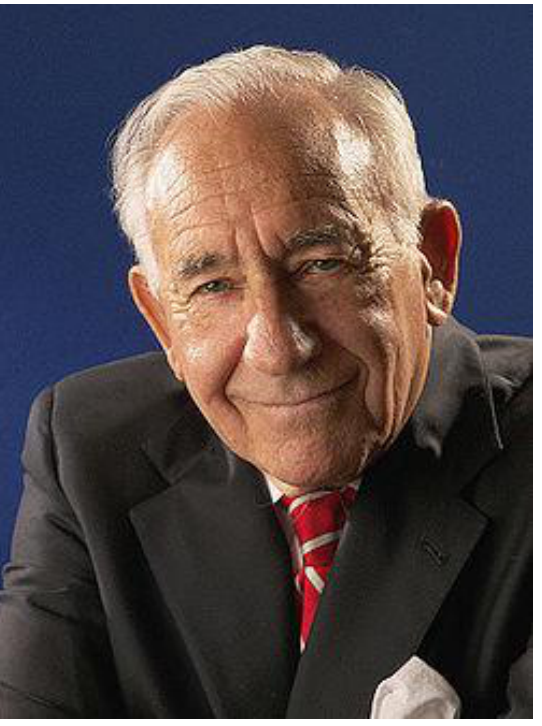
\includegraphics[width=59.22mm,height=199.58mm]{../../images/llm/page_038_img_01.png}%
\end{textblock*}

\end{document}
